\documentclass{beamer}
\mode<presentation>

\usepackage[english]{babel}
\usepackage[latin1]{inputenc}
\usepackage{times}
\usepackage[T1]{fontenc}
\usepackage{graphicx}
\usepackage[justification=centering]{caption}
\usepackage{subcaption}
\usepackage{url}
\usepackage{setspace}
\usepackage{color}
\usepackage{algorithm2e}

\usepackage{listings}
\lstset{breaklines=true}
%\lstset{upquote=true}
\lstset{basicstyle= \small}%\footnotesize}

\usepackage{tikz}
\usetikzlibrary{trees}

\usepackage{pgfpages}

\addtobeamertemplate{navigation symbols}{}{%
    \usebeamerfont{footline}%
    \usebeamercolor[fg]{footline}%
    \hspace{1em}%
    \insertframenumber%/\inserttotalframenumber
}

\AtBeginSection[]{
  \begin{frame}
  \vfill
  \centering
  \begin{beamercolorbox}[sep=8pt,center,shadow=true,rounded=true]{title}
    \usebeamerfont{title}\insertsectionhead\par%
  \end{beamercolorbox}
  \vfill
  \end{frame}
}

\usepackage{hyperref}

\newcommand{\orka}{\textit{Orka}}
\newcommand{\petra}{\textit{PETrA}}

\newcommand{\monkeyrunner}{\texttt{monkeyrunner}}
\newcommand{\apk}{\texttt{apk}}
\newcommand{\logcat}{\texttt{logcat}}
\newcommand{\netstats}{\texttt{netstats}}

\newcommand{\lv}{Linares-Vasquez et al.}
%\setbeameroption{show notes on second screen=left}
%\setbeameroption{show only notes}
\setbeameroption{show notes}
\title[Project presentation]{\textsc{Hardware-usage accounting and source-line level energy estimates on Android}}
\author{Alexandre \textsc{Cornet}\\ {\footnotesize supervised by Dr. Anandha \textsc{Gopalan}}}
\institute{Eighth International Conference on Smart Grids, Green Communications and IT Energy-aware Technologies}
\date{May 2018}
%\pgfdeclareimage[height=0.5cm]{university-logo}{figures/imperial.pdf}
%\logo{\pgfuseimage{university-logo}}
\begin{document}
\tikzstyle{every node}=[draw=black,thick,anchor=west]
\tikzstyle{selected}=[draw=red,fill=red!30]
\tikzstyle{optional}=[dashed,fill=gray!50]
\begin{frame}
\titlepage
\end{frame}
%
\iffalse
\begin{frame}
\framtitle
\tableofcontents%[pausesections]
}
\end{frame}
\fi
%
%%%%%%%%%%%%%%% PROBLEM
%
\section*{Problem}
% FIXME text box on top of frame
\note{
TIMER\\
one page - def continu
\\~\\
Intro\\
Energy optimization of Android application\\
How we approached the two specific pbs of...
\\~\\
Why are these relevant?\\
App dev doing well\\
But keep getting this}
\begin{frame}{Motivations}
\begin{columns}
\begin{column}{0.5\textwidth}
\begin{figure}
        
\includegraphics[width=\textwidth]{figures/angry_feedback_1.png}
\end{figure}
\end{column}
\begin{column}{0.5\textwidth}
\begin{figure}
        
\includegraphics[width=\textwidth]{figures/angry_feedback_2.png}
\end{figure}
\end{column}
\end{columns}
\note{
angry feedback regarding the energy consumption of your app\\
realize energy efficiency matters\\
decide to optimise your code for it
\\~\\
before discussing your options...\\
TE because
}
\end{frame}
%
\begin{frame}{An asynchronous power-behaviour: Tail-energy}
\note{
DEFINITION
\\~\\
power behaviour can be modelled using a \alert{power state machine}\\
always \alert{two states at least}
\\~\\
for many mobile components, a \alert{third state}, the tail-state\\
entered after a workflow has been processed\\
stay in that state for a definite time, \alert{tail-time}\\
spend \alert{tail-energy}
\\~\\
significant fraction of the energy drain comes from TE\\
this behaviour is highly relevant to our pb
}
\begin{columns}
\begin{column}{0.5\textwidth}
\begin{definition}
\begin{itemize}
\item A component exhibits \alert{tail-behaviour} if it stays in a high power-state \alert{after} processing a workflow.
\end{itemize}
\end{definition}
\end{column}

\begin{column}{0.5\textwidth}
\begin{figure}
	\centering
	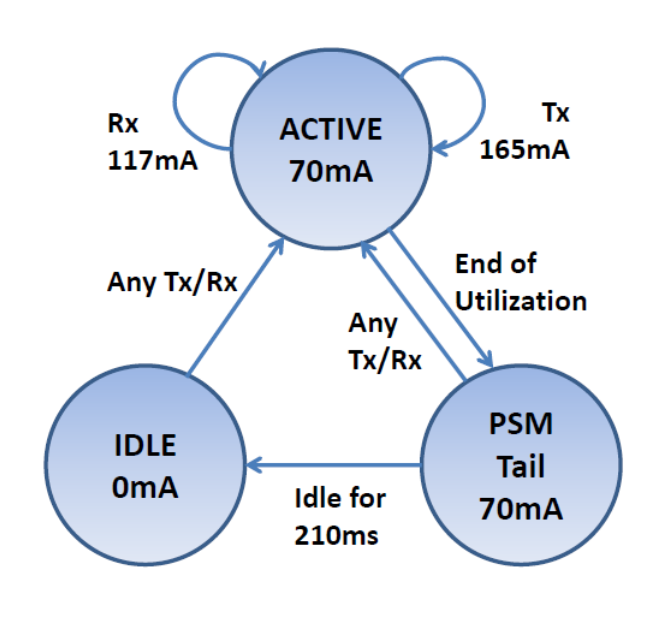
\includegraphics[width=\textwidth]{figures/wifi_statemachine.png} 
	\caption{Power-state machine of a Wi-Fi antenna  \cite{Ding:2013:CMI:2465529.2466586}}
\end{figure}
\end{column}
\end{columns}
\end{frame}
%
%
\begin{frame}{Related work: Energy-profilers (1/2)}
\begin{itemize}
\item \alert{Hardware based} profilers rely on power measurement platforms.
\item \alert{Model based} profilers embed these power measurements in off-line models.
\item \textit{vLens} \cite{li2013calculating} (hardware-based) and \textit{eprof} \cite{pathak2012energy} (model-based):
\begin{itemize}
\item Rely on instrumentation
\item Generate \alert{source-line level estimates}
\item Account for \alert{tail-energy}: \textit{eprof} generates \texttt{(utilisation\_draw, 
tail\_mode\_draw)} tuples
\end{itemize}
\end{itemize}
\note{
Back to our pb,
Best option is definitely to use an energy profiler, able to highlight...
divided into 3 categories\\
DEFINITION Hardware / model based\\
~\\
Interesting contributions: vLens, eprof\\
%Eprof: \alert{models component energy behaviour using FSM}\\
Why I mentioned TE\\
By design, lead to a financial and practical overhead
}
\end{frame}
%
\begin{frame}{Related work: Energy-profilers (2/2)}
\begin{itemize}
\item \alert{Software-based} profilers: portable and widely accessible
\item \textit{PETrA} \cite{petra}:
\begin{itemize}
\item Lightweight: only needs the application and a test script
\item \alert{Relies on \textit{Android}} tools to collect the execution trace and energy related logs
\item Doesn't account for tail-energy
\item \alert{Method-level} feedback
\end{itemize}
\end{itemize}
\note{
software-based tools introduced to move away from this requirements\\
~\\
PETRA\\
%Also uses a FSM modeling of energy behaviour\\
No tail energy, so \alert{ignoring a significant fraction} of the drain\\
Method level feedback: but \alert{still the responsibility of the developers} to find the energy bugs\\
Recent tool, I was in contact with the team\\
%+ not available as this work started\\
So, what's missing to solve our problem?}
\end{frame}
%
%
\begin{frame}{What's missing?}
An energy-profiler:
\begin{enumerate}
\item \alert{Software-based}
\item Providing \alert{source-line level} estimates
\item Providing hardware-usage and \alert{tail-energy} accounting
\end{enumerate}
\note{
%After the reviewing the state-of-art literature, my opinion was there is \alert{a need for}...
Whta's missing?\\
~\\
going to explain how we delivered this
}
\end{frame}
%
%%%%%%%%%%%%%%% ORKA
%
\section{Orka}
\note{introduce orka\\
software based tool I extended to implement these requirements}
\begin{frame}{\orka{}: overview}
\begin{itemize}
%\item Input: Tested \apk{} file and \monkeyrunner{} test script
%\item Output: Energy estimates at the method-level`
\item \lv{} \cite{linares2014mining} computed the energy costs of 800 API calls
\begin{itemize}
\item Calls to the Android API are the most energy greedy
\end{itemize}
\item Main assumption:
\begin{align*}
cost(line) &=  \sum_{API \in line} cost(API) 
\end{align*}
%cost(routine) &= \sum_{line \in routine} cost(line) \\
\item Rely on \alert{instrumentation} and on the Android \alert{emulator}
\end{itemize}
\note{
Based on \alert{LV work}, it approximates\\
Based on this assumption, it \alert{tallies calls} to the A. API\\
Cost method = sum cost line\\
Rely on \alert{instrumentation}
}
\end{frame}
%
%
\begin{frame}{\orka{}: workflow}
\begin{figure}
        \includegraphics[width=\textwidth]{figures/orkaworkflow.pdf}
\end{figure}
\note{
Instrumentation: insert call to the Log API to record information needed to compute costs}
\end{frame}
%
%%%%%%%%%%%%%%% SOURCE-LINE
%
\section{Source-line level energy estimates}
\note{
How we were able to compute source line level energy estimates based on these assumptions\\
Goal: generates a reconstructed source-code with line-level estimates
}
%
%
\begin{frame}{What's needed to solve this?}
\begin{itemize}
\item We want to compute :
$$cost(line) = \sum_{API \in line} cost(API)$$
\item $cost(API)$ is given by \lv{} \cite{linares2014mining} work.
\item Hence, we need to compute $\{API \in line\}$
\item Possible to derive this from the execution trace.
\end{itemize}
\end{frame}  
%
%
\begin{frame}[fragile]{Execution trace}
\begin{figure}
\centering
%
\begin{subfigure}[t]{0.45\textwidth}
\caption{\texttt{java} code of two example functions}
\centering
\begin{lstlisting}[numbers=left]
public void a() {
  API1();
  call b();
  return;
}
public void b() {
  API2();
  return;
}
\end{lstlisting}
\end{subfigure}
%
\begin{subfigure}[t]{0.5\textwidth}
\centering
\caption{\logcat{} output produced by the execution of routine \texttt{a}}
\begin{lstlisting}
entering a
API call l2 API1
invoking subroutine l3 b
entering b
API call l7 API2
exiting b
exiting a
\end{lstlisting}
\label{fig:exlogcat3}
\end{subfigure}
\end{figure}
\note{
Let's look at a simple example\\
DESCRIBE FUNCTIONS\\
DESCRIBE COST ATTRIBUTION\\
All information is contained is this stack trace
}
\end{frame}  
%
%
\begin{frame}[fragile]{Code injection}
\begin{figure}
\caption{Injected functions}
\centering
\begin{subfigure}[t]{0.49\textwidth}
\centering
\begin{lstlisting}
public void a() {
  Log("entering a")
  Log("API call l2 API1")
  API1();
  Log("invoking subroutine l3 b")
  call b();
  Log("exiting a")
  return;
}
\end{lstlisting}
\end{subfigure}
%
\begin{subfigure}[t]{0.49\textwidth}
\centering
\begin{lstlisting}
public void b() {
  Log("entering b")
  Log("API call l7 API2")
  API2();
  Log("exiting b")
  return;
}
\end{lstlisting}
\end{subfigure}
\end{figure}
\note{
What do we need to inject\\
method enter and exit\\
API invocation with line\\
line of subroutines invocation \\
Injection process relies on \alert{bytecode analysis}\\
Application is decompile, injected and recompiled\\
What is Log
}
\end{frame} 
%
%
\begin{frame}[fragile]{Analyser} % Replay of Logcat and call stacks
%\begin{columns}
%\begin{column}{0.5\textwidth}
\begin{itemize}
\item Replay the execution trace
\item Maintain an in memory version of the call stack, including the line of each call
\item This way, able to tally the API calls within each line
\end{itemize}
\iffalse
\end{column}
%
\begin{column}{0.4\textwidth}
\begin{figure}%[language=java]
\centering
\begin{lstlisting}[numbers=left]
public void a() {
  API1();
  call b();
  return;
}
public void b() {
  API2();
  return;
}
\end{lstlisting}
\end{figure}
\begin{tabular}{c | c}
   & API2 \\
   API1 &  b, 7\\
  a, 2 & a, 3 
\end{tabular}
\end{column}
\end{columns}
\fi
\note{
}
\end{frame}  
 %
 %
\begin{frame}[fragile]{Final output}
\centering
%[caption=Example of reconstructed source code providing fine-grained guidance]
{\tiny%\footnotesize
\begin{lstlisting}
method RecList.onCreate, Average cost: 0.0197754308, Calls: 1.0
   2.64% l-1
   1.45% l192 calling RecList.InitRepeatButton
   0.88% l227 calling RecList.InitThemedButtons
   0.57% l229 calling Pref.getPlayingFilePath
  29.04% l247 calling RecList.updateSongList
  21.80% l257 calling android.os.Bundle.getString
  21.80% l258 calling android.os.Bundle.getString
  21.80% l260 calling android.os.Bundle.getString
\end{lstlisting}}
\note{
DESCRIBE\\
for clarity, uses \alert{relative cost}
}
\end{frame}
%
%%%%%%%%%%%%%%% HARDWARE
%
\section{Hardware-usage and tail-energy accounting}
\note{
Focus on probably the most significant contribution of this work
}
\begin{frame}[fragile]{Problem}
\begin{block}{Aims}
\begin{itemize}
\item Map hardware-usage back to the code
\item Account for tail-energy
\end{itemize}
\end{block}
%
\begin{block}{Specification}
\begin{itemize}
\item Produce energy tuples
\end{itemize}
%MainActivity.<init> {ACTIVE: 0.0, IDLE: 0.01, TAIL: 0.0}
\begin{lstlisting}`
MainActivity$SendGet.run {ACTIVE: 1.57, IDLE: 0.84,
  TAIL: 1.62}
\end{lstlisting}
\end{block}
%
\begin{block}{Simplifications}
\begin{itemize}
\item Only for Wi-Fi, at the method level
\item Focus on time ($E= P \Delta_t$)
\end{itemize}
\end{block}
\note{
MAP: e.g Wifi is drain the battery: where does this happen?
\\~\\
For one method, tuples represent the \alert{time spent in each mode } by a component, which is attributed to the method\\
Because of the method XX, the component spent ...
\\~\\
I/O consumes the most energy -- only Wi-FI\\
Simple relation between time and energy -- focus on time
}
\end{frame}
%
%
\begin{frame}{Technical challenges}
\begin{block}{Goal}
\begin{itemize}
\item \alert{Correlate} the Wi-Fi energy activity with routine calls
\end{itemize}
\end{block}
\begin{block}{Requirements}
\begin{itemize}
\item Monitoring the call-stack
\item Monitoring the power state of Wi-Fi
\end{itemize}
\end{block}
\note{
Refer to FSM\\
call-stack: know which routines are executed at any time\\
%Leave call-stack to QA\\~\\
Wifi power state: Not possible to monitor directly as not logged by OS\\
}
\end{frame}
%
%
\begin{frame}[fragile]{Monitoring the power state of Wi-Fi}
% FIXME two col, add state machine
\begin{itemize}
\item We need to monitor what triggers transitions: \alert{network traffic}.
\item Leverage \texttt{proc/net/xt\_qtaguid/stats}
\end{itemize}
\vskip0pt plus.5fill
%[frame=single]
\begin{lstlisting}
idx iface uid_tag_int cnt_set rx_bytes rx_packets tx_bytes tx_packets
2 wlan0 0 0 200888 1096 79636 888
3 wlan0 0 1 0 0 0 0
\end{lstlisting}
\note{
OS logs the number of bytes send and received by each application\\
able to fetch this file every 50ms\\
hence able to monitor traffic with a 50ms \alert{sampling period}\\
thanks to this, I can \alert{deduce when Wi-Fi switches}  from one state to another
}
\end{frame}
% FIXME
%
%
\begin{frame}{Implementing the power state-machine}
\begin{figure}
% FIXME better breakdown
	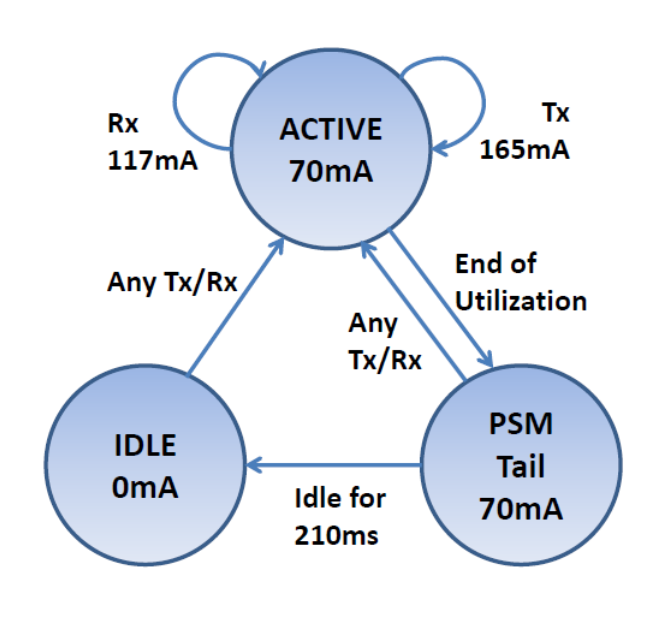
\includegraphics[height=0.6\textheight]{figures/wifi_statemachine.png} 
	\caption{Power-state machine of a Wi-Fi antenna}
\end{figure}
\note{
leave more detailed speudo QA\\~\\
High level idea:\\
if any traffic: active\\
no traffic from active: tail\\
if in tail mode: check for time condition
}
\end{frame}
%
% 
\begin{frame}[fragile]{Network analyser: principle}
\begin{columns}
\begin{column}{0.5\textwidth}
% 09-04 12:52:26.642 1474 9092 I orka: Ind
\begin{lstlisting}
12:52:26.642 entering foo
12:52:26.742 	...
12:52:26.842 entering bar
12:52:26.942 	...
12:52:27.042 exiting bar
12:52:27.142 exiting foo
\end{lstlisting}
\end{column}
\begin{column}{0.5\textwidth}
\begin{lstlisting}
1503657227.589833 ACTIVE
1503657227.644556 TAIL
1503657227.681700 TAIL
1503657227.716493 TAIL
1503657227.753575 TAIL
1503657227.864556 IDLE
\end{lstlisting}
\end{column}
\end{columns}
\vskip0pt plus.5fill
\begin{itemize}
\item Replay both logs
\item Tally time spent in each mode for all methods
\end{itemize}
\note{
merge sort\\
leave algo for QA\\
\vspace{2cm}
let's log processed until t0, state up to date\\
let's fetch next entry at t0 + delta t\\
state is constant during delta t\\
add delta t in current state to all method in the call stack\\
update state\\
loop
}
\end{frame}
%
%
\begin{frame}[fragile]{Network analyser: results}
\begin{lstlisting}
MainActivity.<init> {ACTIVE: 0.0, IDLE: 0.01,
  TAIL: 0.0}
MainActivity$SendGet.run {ACTIVE: 1.57, IDLE: 0.84,
  TAIL: 1.62}
\end{lstlisting}
\end{frame}
%
\begin{frame}[fragile]{Evaluation}
\begin{itemize}
\item Aim: verify high-level expectations
\begin{itemize}
\item Good energy efficiency for dense network traffic
\item Efficiency decreases when period gets close to tail-time
\end{itemize}
\item Tested against a custom app, sending network requests at a chosen frequency
\item Orka is able to detect the method sending the request.
\item Need to improve accounting policy: \alert{last-trigger policy}
\end{itemize}
\note{
 Aim: verify high level exp\\
 using custom app sending GET every T ms\\
 Highlighted \alert{too simple accounting policy}
}
\end{frame}
%
%
%%%%%%%%%%%%%%% CONCLUSION
%
\section{Conclusion}
\iffalse
\begin{frame}{Future work}
\begin{itemize}
\item Tail-energy: implement last-trigger policy and extend to other components
\item Improve the injector
\item Improve accuracy
\end{itemize}
\note{
injector: \alert{single point of failure}, need to \alert{broaden its reach}\\
}
\end{frame}
\fi
%
%
\begin{frame}[allowframebreaks]
        \frametitle{References}
        \bibliographystyle{plain}
        {\footnotesize \bibliography{references.bib} }
\end{frame}
%
%
\begin{frame}
  \vfill
  \centering
  \begin{beamercolorbox}[sep=8pt,center,shadow=true,rounded=true]{title}
    \usebeamerfont{title}Thank you.\par%
  \end{beamercolorbox}
  \vfill
\end{frame}
%
%%%%%%%%%%%%%%% OTHER WORK
%
\section{Appendix}
\note{
other important contributions\\
Important efforts were made to \alert{refactor}\\
in order to \alert{ease the implementation} of extensions\\
\alert{improve usability}\\
leave to QA
}
%
%
\begin{frame}{Evaluation of \orka{}}
\begin{itemize}
\item Aim: perform evaluation during the development cycle
\item Generated reference results using \petra{} \cite{petra}
\item To this end, built a \alert{test environment} for \orka{}
\item High error rate on average
\end{itemize}
\note{
\alert{made possible by petra} = software based tool released in March\\
test env allows to enter one command to run the eval\\
= generate results with orka on a set of test applications\\
then compare\\~\\
high error rate but too late to investigate
}
\end{frame}
%
\begin{frame}{Architecture}
\begin{figure}
\centering
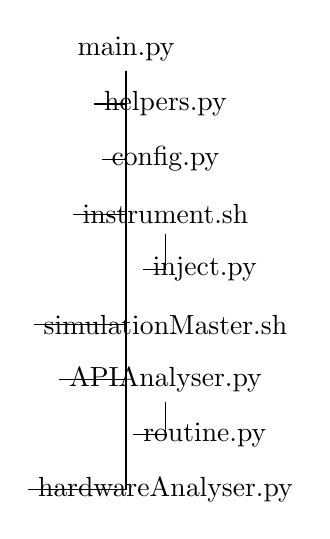
\begin{tikzpicture}[%
  grow via three points={one child at (0.5,-0.7) and
  two children at (0.5,-0.7) and (0.5,-1.4)},
  edge from parent path={(\tikzparentnode.south) |- (\tikzchildnode.west)}]
  \node {main.py}
    child { node {helpers.py}}
    child { node {config.py}}
    child { node {instrument.sh}
    	child { node {inject.py}}}
    child [missing] {}
    child { node {simulationMaster.sh}}
    child { node {APIAnalyser.py}
    	child { node {routine.py}}}
    child [missing] {}
    child { node {hardwareAnalyser.py}};
\end{tikzpicture}
\caption{\orka{}'s design}
\label{fig:design}
\end{figure}
\end{frame}
%
%
\begin{frame}[fragile]{Monitoring the call-stack}
\note{
Logs when routines start and terminate\\
initial version only logs when method enter\\
changed the output format of orka\\
}
\begin{columns}
\begin{column}{0.4\textwidth}
\begin{itemize}
\item Extended the injector to \alert{log when methods return}
\item Used \logcat{} in \texttt{threadtime} mode to \alert{include timestamps}
\end{itemize}
\end{column}
\begin{column}{0.6\textwidth}
% 09-04 12:52:26.642 1474 9092 I orka: Ind
\begin{lstlisting}
12:52:26.642 entering foo
12:52:26.742 	API call api1
12:52:26.842 entering bar
12:52:26.942 	API call api2
12:52:27.042 exiting bar
12:52:27.142 exiting foo
\end{lstlisting}
\end{column}
\end{columns}
\end{frame}
%
%
\begin{frame}{Network monitoring: algorithm}
\begin{small}
\begin{algorithm}[H]
%\KwIn{Active ADB connection to an actual device}
\KwOut{Logs of the energy states of the Wi-Fi antenna}
Get first network statistics $S_0$ at current time $t_0$\;
$state \leftarrow \texttt{IDLE}$\;
\While{True}{
Get network statistics $S_1$ at current time $t_1$\;
\uIf{$S_0 \neq S_1$}
{$state \leftarrow \texttt{ACTIVE}$\;}
\ElseIf{state = \texttt{ACTIVE}}{$state \leftarrow \texttt{TAIL}$\;$tail_{start} \leftarrow t_0$\;}
\If{$state = \texttt{TAIL}$ {\normalfont \textbf{and}} $t_1 - tail_{start} \geq tail_{time}$}
{Log $(t_0, state)$\;
$t_0 \leftarrow tail_{start} + tail_{time}$\;
$state \leftarrow \texttt{IDLE}$\;}
Log $(t_0, state)$\;
$t_0 \leftarrow t_1$, $S_0 \leftarrow S_1$\;
}
\end{algorithm}
\end{small}
\note{
if any traffic: active\\
no traffic from active: tail\\
if in tail mode: check for time condition
}
\end{frame}
%
%
\begin{frame}[fragile]{Network monitoring: results}
\begin{lstlisting}
1503657227.287407 ACTIVE
1503657227.323574 TAIL
1503657227.359771 TAIL
1503657227.394717 TAIL
1503657227.428777 ACTIVE
1503657227.467203 TAIL
1503657227.518874 ACTIVE
1503657227.589833 ACTIVE
1503657227.644556 TAIL
1503657227.681700 TAIL
1503657227.716493 TAIL
1503657227.753575 TAIL
1503657227.789498 TAIL
1503657227.829724 TAIL
1503657227.864556 IDLE
1503657227.882524 IDLE
\end{lstlisting}
\end{frame}
%
%
\begin{frame}{Network analyser: algorithm}
\begin{small}
\begin{algorithm}[H]
\KwIn{\logcat{} and \netstats{} traces}
\KwOut{Energy tuples describing the Wi-Fi activity for each injected routine}
Initialise routine cost tuples\;
Initialise call stack\;
$state \leftarrow \texttt{IDLE}$\;
\While{{\normalfont Log files contain entries left to process}}{
Get the non-processed entry with the smallest time-stamp\;
Add time spent since the last update in the current state to all routines in the stack\;
Update the call stack if the entry comes from \logcat, otherwise update the $state$\;
}
\end{algorithm}
\end{small}
\note{
let's log processed until t0, state up to date\\
let's fetch next entry at t0 + delta t\\
state is constant during delta t\\
add delta t in current state to all method in the call stack\\
update state\\
loop
}
\end{frame}
%
%
\begin{frame}{Summary}
This work stands as the first software-based tool:
\begin{enumerate}
\item Accounting for \alert{tail-energy}
\item Providing \alert{source-line level} energy estimates
\item Available as an \alert{open-source} application
\end{enumerate}
\vskip0pt plus.5fill
{\small \orka{} is available at \url{https://github.com/acornet/orka}}
\note{\alert{what I'd like to leave you with}}
\end{frame}
%
%
\end{document}
